Powerful AI instrumentation relies on {\bf co-design} -- the idea that system constraints, algorithm development, and hardware implementation inform and guide each other in complementary ways. 
%Development of physics experiments are typically driven by this principle which starts from the physics requirements and drills down to the technical specifications of the apparatus. 
AI\textsuperscript{3}'s co-design ecosystem is illustrated in Fig.~\ref{fig:codesign}. In addition to hard real-time latency constraints, other experimental challenges provide further constraints.  For example, sensors in harsh and complex environments may have strict power limits or need to operate in high radiation or cyrogenic environments.  Therefore, we will explore hardware co-design for various technologies from FPGAs to custom integrated circuits like ASICs and neuromorphic chips to ultra-low power photonics and opto-electronic devices to exotic memristive and organic-electronic hybrids. 


\subsubsection{Algorithm-Architecture Co-Design} \label{sec:HwAlgo}

\begin{wrapfigure}{r}{0.5\textwidth}
\centering
\vskip-40pt
  {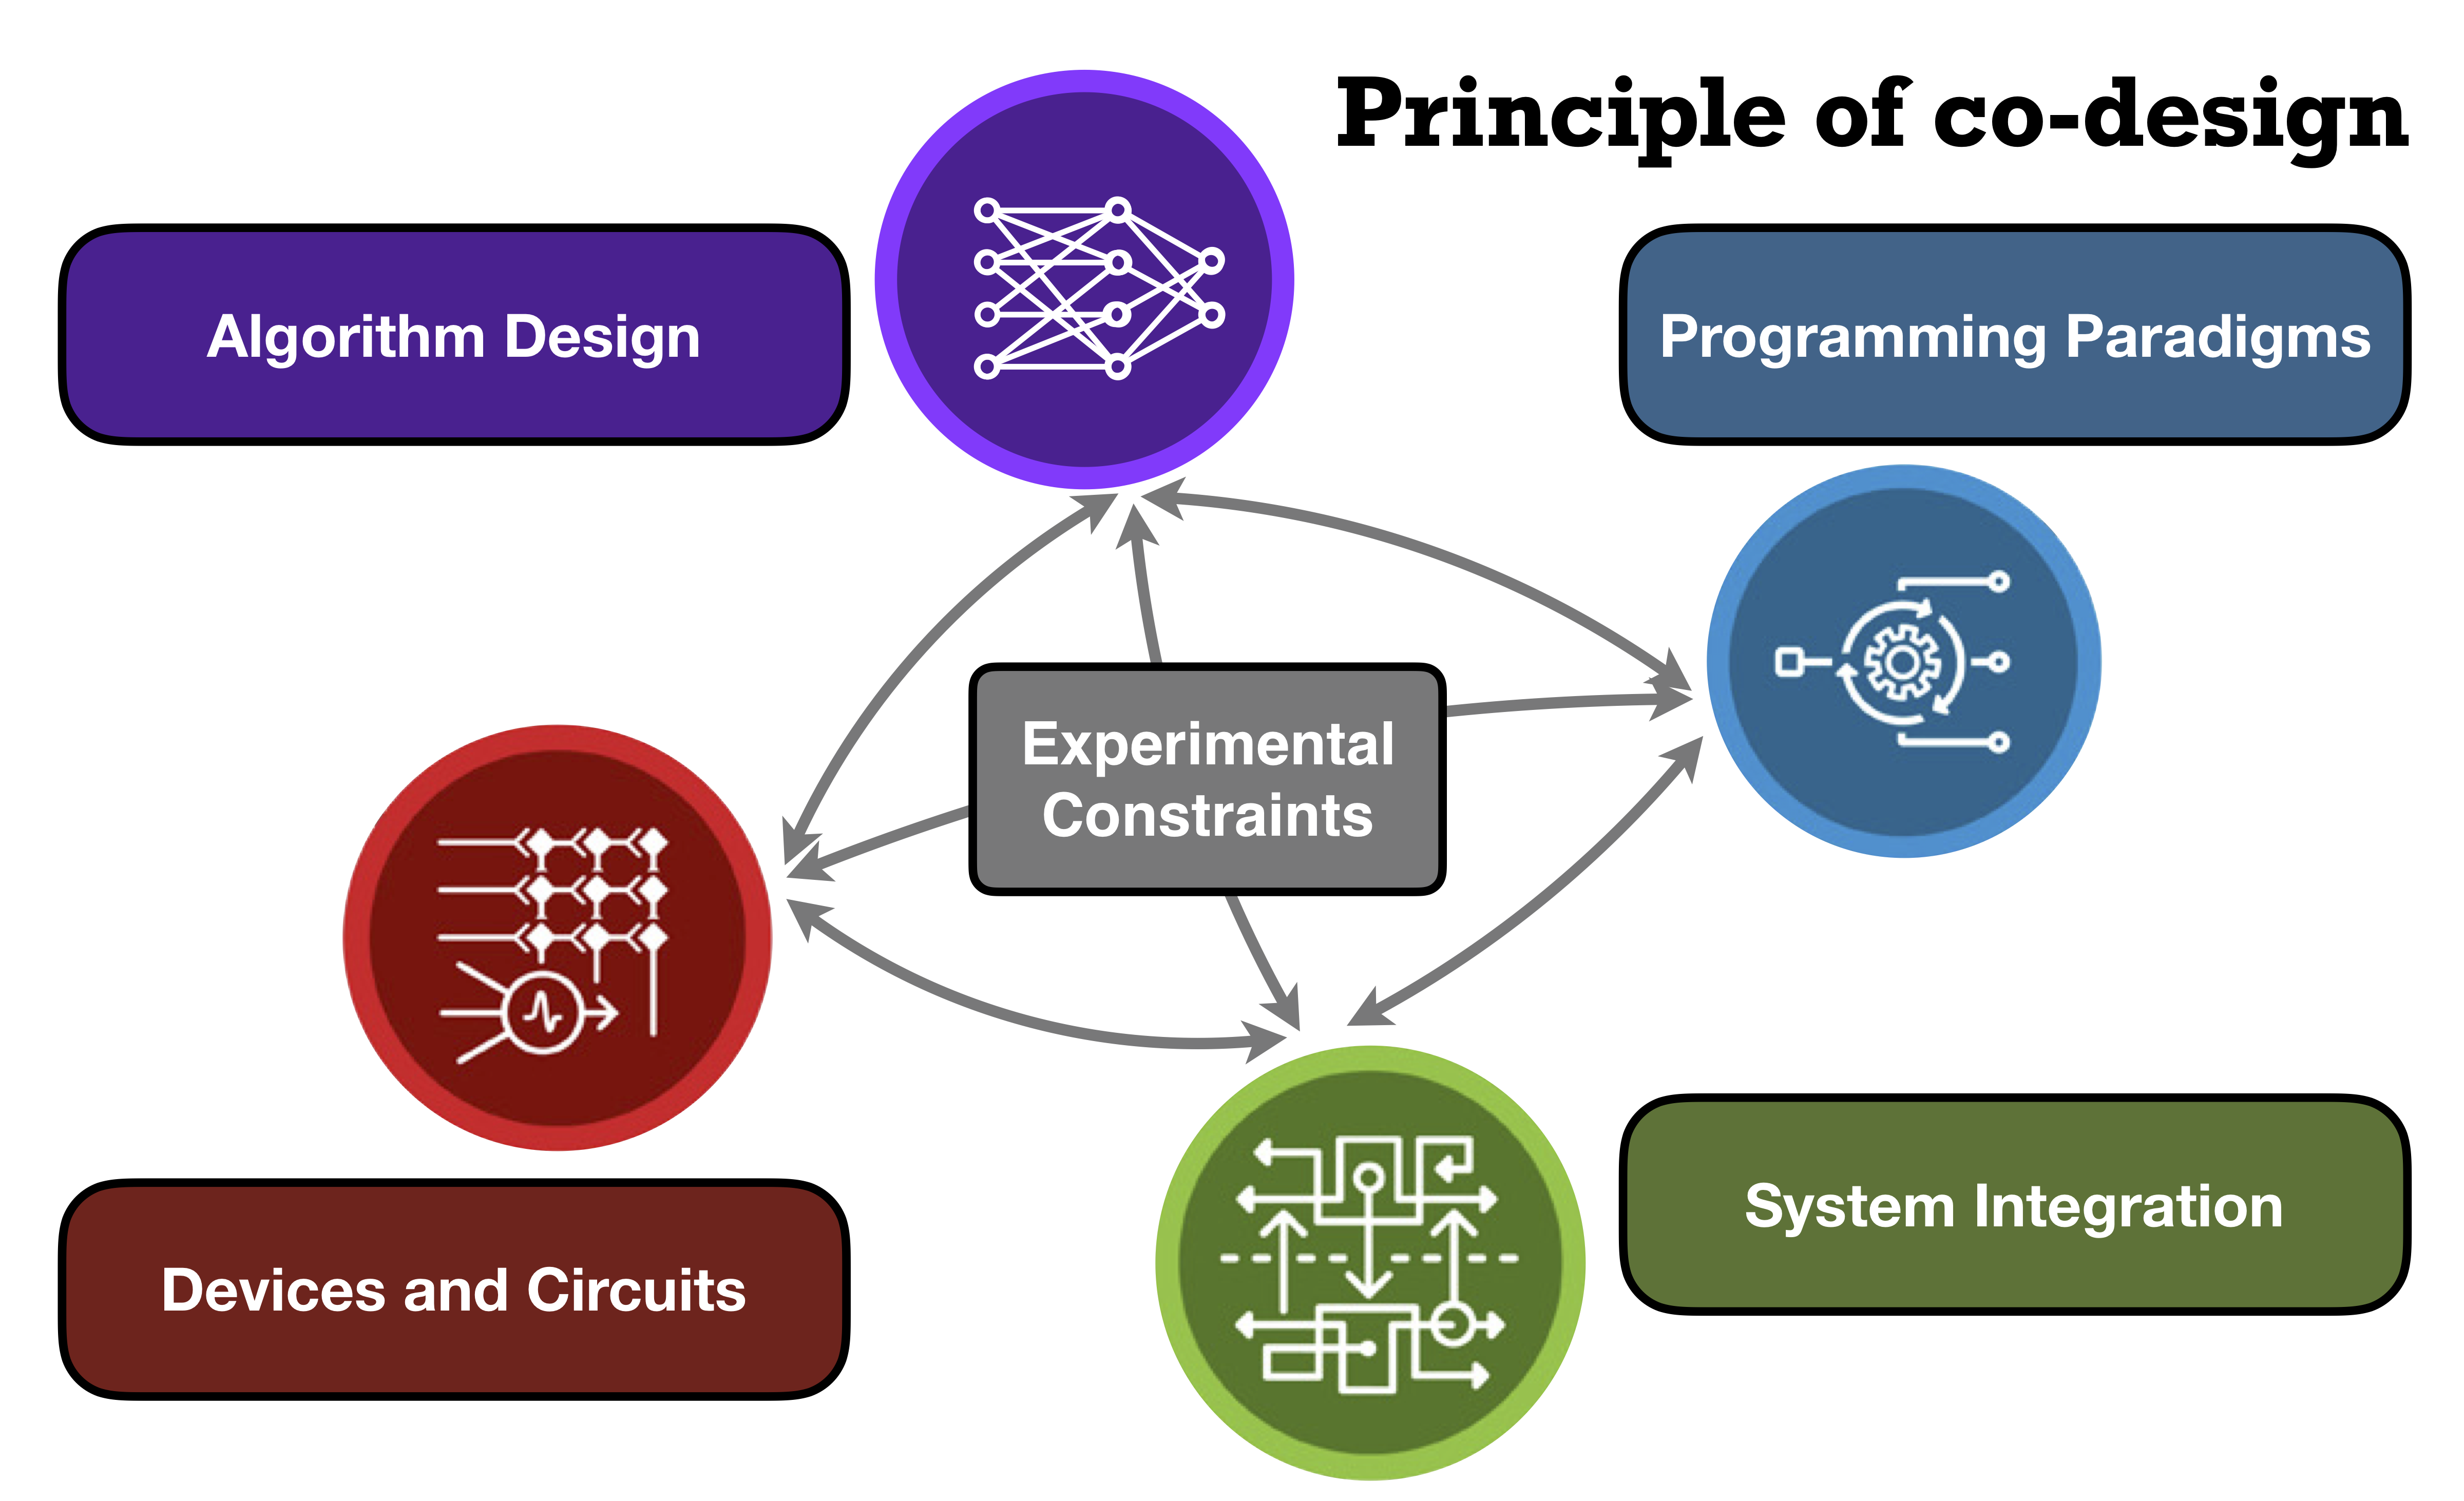
\includegraphics[keepaspectratio, width=0.5\textwidth]{proposal/img/codesign.png}}
  \caption{Hardware co-design principle which coherently integrates all levels of experimental design.}
  \label{fig:codesign}
  \vskip-15pt
\end{wrapfigure}
The development of efficient AI implementations in hardware begins with algorithm performance and design.
%Section~\ref{sec:AI} details the many AI methods that are required to attain our significant physics goals.  
As we consider how to implement the AI hardware in high-rate and resource-constrained environments, there are important considerations in building the most efficient systems. We must consider the size and structure of the AI computation. Neural networks are generally characterized through a number of multiplication and addition operations using fitted parameters (weights) determined during the training procedure. By reducing both the number of mathematical operations and how often the weights need to be accessed, the algorithm can be made more efficient.  Further, the precision at which the calculations are performed is also important.
%The optimization of the number of operations and their precision and the number of parameters can greatly reduce the resources required to perform a given AI computation.  
{\bf SP Duarte} and collaborators~\cite{Duarte:2018ite} explored the design space of AI algorithm performance while reducing the calculation precision and removing unimportant calculations (pruning/compression).  However, as neural network architectures become more complex and varied, this optimization must be understood in greater detail. New techniques, such as energy-aware pruning, can be used to improve the energy consumption directly~\cite{DBLP:journals/corr/YangCS16a}.

Just as important is the conception of the AI architecture. AI algorithms are over-parameterized universal function approximators. Directly connected to our research of physics-inspired learning (see Section~\ref{sec:AI}),  embedding our own physics knowledge into the neural network design can drastically reduce the number of parameters in a given neural network algorithm.  For example, exploiting physical symmetries in neural networks has been shown to reduce the computational complexity, e.g., tensor field networks that incorporate rotation- and translation-equivariance for 3D point cloud data~\cite{thomas2018tensor}. {\bf SP Su's} work has also demonstrated that learning a spectral convolutional neural network may achieve isometric invariance of geometric data. 

In order to create optimal AI hardware implementations, both of the above techniques are required.  First, we can reduce the computational complexity of the AI algorithm by embedding our physics knowledge into the network design. Then, we can further optimize the efficiency by adapting the algorithm for custom hardware while minimizing the energy footprint of calculation and maintaining performance. A central aspect of AI\textsuperscript{3}'s research program is to understand the strengths and limitations of different AI algorithms and techniques (from physics-inspired networks to transfer learning, compression, and autoencoders), including their ultimate performance, computational complexity, and applicability in hardware. {\bf SP Duarte} will lead this project in collaboration with {\bf SP Su}.

%%%%%%%%%%%%%%%%%%%%%%%%%%%%%%%%%%%%%%%%%%%%%%%%%%%%%%%%%%%%%%%%%%%%%%%%%%%%%%%%%%%%%%%%%%%%%%%
%%%%%%%%%%%%%%%%%%%%%%%%%%%%%%%%%%%%%%%%%%%%%%%%%%%%%%%%%%%%%%%%%%%%%%%%%%%%%%%%%%%%%%%%%%%%%%%

%\newpage 
\subsubsection{Programming Paradigms and Tools} \label{sec:Programming}


\begin{wrapfigure}{r}{0.6\textwidth}
\centering
\vskip-15pt 
  %\fbox
  {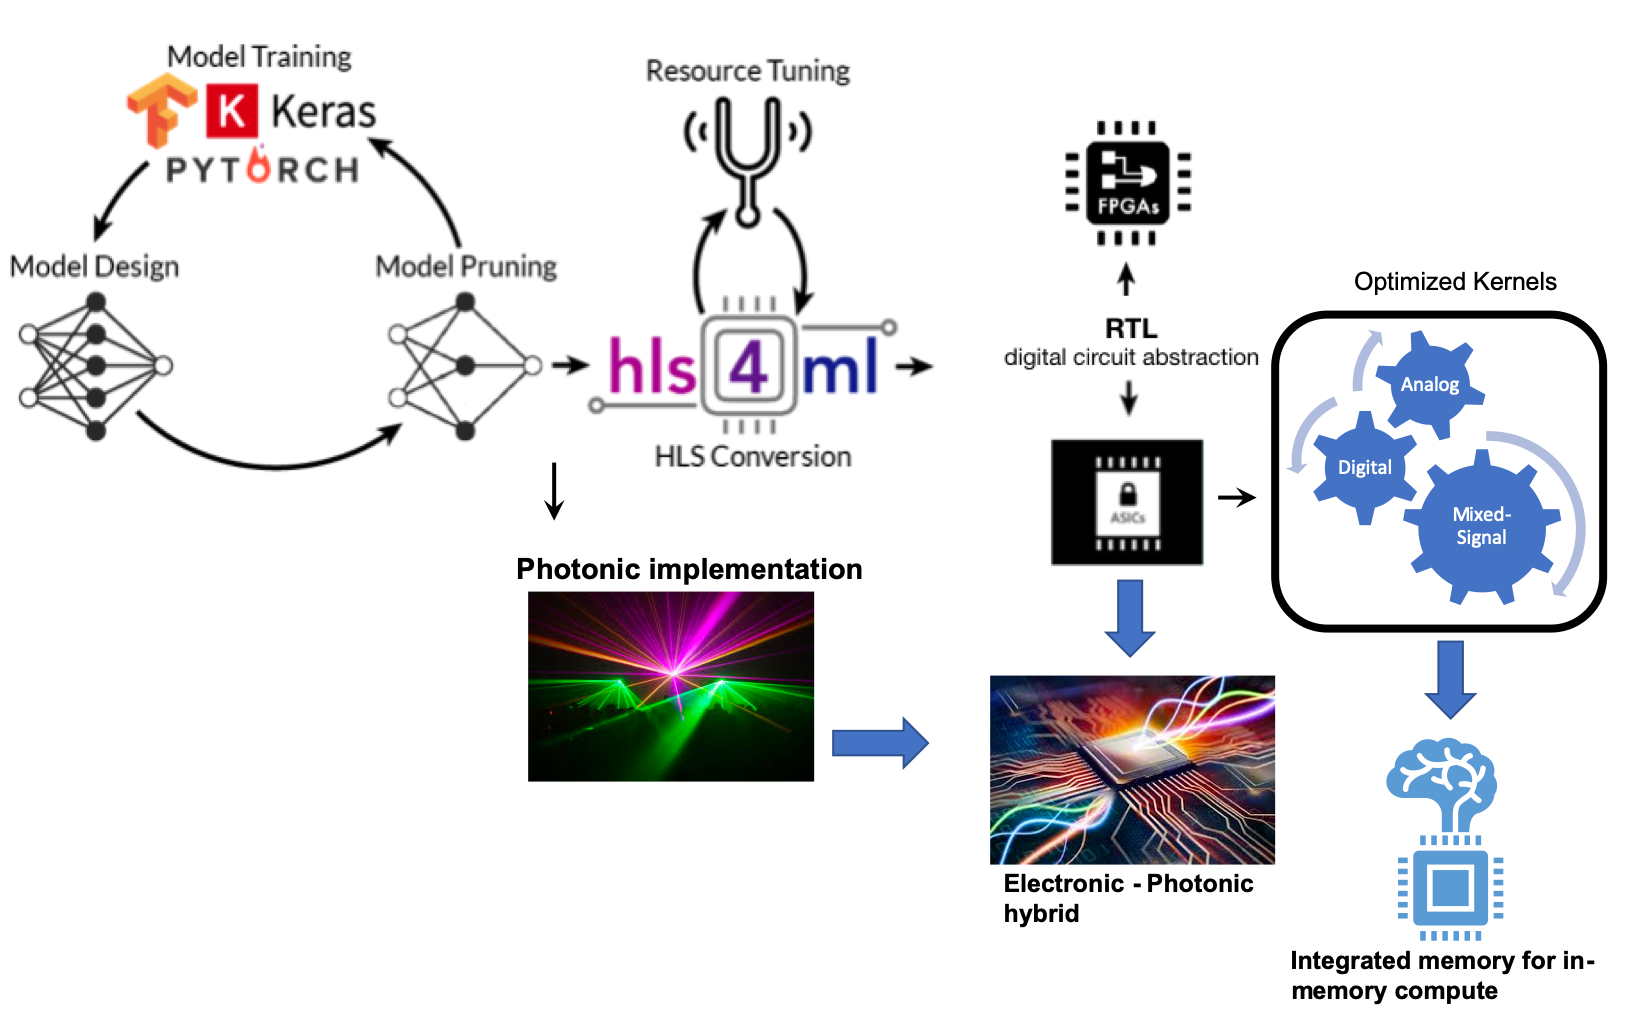
\includegraphics[keepaspectratio, width=0.6\textwidth]{proposal/img/ProgrammingFlow.png}}
  \caption{Full example workflow from HLS programming paradigms to hybrid solutions.}
  \label{fig:programming}
  \vskip-10pt 
\end{wrapfigure}
AI\textsuperscript{3}'s main goal in developing programming paradigms and tools will be to increase accessibility of hardware implementations of  algorithms in order to accelerate the development cycles for AI instrumentation. Mature programming tools are absolutely vital to wider deployment and adoption which will in turn improve the overall physics design process. Furthermore, widely accessible programming paradigms will be instrumental for easy and quick adoption by a large community of learners that can be trained for the future workforce in AI instrumentation for physics. %AI\textsuperscript{3} is targeted towards experimental physics constraints, but the tools will be available to the entire design automation community and for developing solutions in other domains. In that regard, 
AI\textsuperscript{3} will also be responsible for communicating, supporting, and educating developers and users. 
%Our plans on translating AI\textsuperscript{3}'s innovations on tool building and methodologies to the broader community will be further discussed in Section~\ref{sec.collab}.   


We will align our tool development strategies with the unique aspects of AI computation. One of the key features of neural networks are their modularity. This allows us to develop programming paradigms that enable the developer to separate and recombine these specific modular units to build larger neural network architectures. The basic description of the AI circuit implementation, for example, can be in a register-transfer language (RTL), but each kernel would be configurable based on resource, latency, and bandwidth constraints.   
%The integration of the kernels into a cohesive system is the subject of the next section on system design and integration, Section~\ref{sec:Integration}. 
One important aspect to AI\textsuperscript{3}'s research program is the use of higher-level programming paradigms based on low-level hardware representations.  
%Programming languages such as High Level Synthesis (HLS) and OpenCL are {\tt C}-based languages which are used to convert code into Register Transfer Level (RTL) Hardware Description Language (HDL). 
\textbf{SP Duarte} is one of the leading developers of a tool called \hlsfml~\cite{Duarte:2018ite} which takes popular open-source machine learning software frameworks such as {\tt TensorFlow}, {\tt Keras}, and {\tt PyTorch} and converts their model descriptions into high-level synthesis (HLS) code. The HLS code has parameters which tune the performance of the underlying hardware description to customize it for different system constraints.  The \hlsfml~tool then uses HLS tools to create an RTL-HDL description of a given AI algorithm for a specific type of hardware.  Despite being a new software package, this tool has seen widespread adoption in the HEP community and has been successfully used for fully-connected neural networks in LHC trigger applications on FPGAs.  The full workflow of \hlsfml~is depicted in Fig.~\ref{fig:codesign}. \textbf{SPs Hahn and Memik} have also been collaborating in developing HLS-based design methodologies for mapping the TrackletEngine algorithm used as part of Level-1 trigger track finding for CMS at the HL-LHC. 
  %This collaboration led to a better understanding of performance bottlenecks when using a commercial FPGA HLS tool flow and the co-PIs will be transferring their experience on existing HLS flows targeting HEP applications to \textbf{co-PI Duarte's} lab as they explore new programming paradigms suited for this domain collectively.  
While developing HLS tools for AI computation in hardware is an important research goal, HLS is not the only solution for AI algorithm implementation.  
%We will explore the limitations of this approach and develop alternatives, as well as compare them to other published software tools, such as Nengo which is described below. 
We plan to extend the workflow in Fig.~\ref{fig:programming} to allow for different types of AI algorithm kernels, domains, and hardware. As an example, EM applications require recurrent neural network structures to optimally interpret their time-ordered data; and \hlsfml~does not yet support those types of recurrent structures.  Further, to support the entire community, it is necessary to support other hardware types.  This includes other custom designs, i.e., Photonic Integrated Circuits (ICs), Digital and  Mixed Mode ASICs. ASICs are particularly important across physics because often experimental instrumentation must operate in extreme and harsh environments, such as high radiation and cryogenics, and off-the-shelf FPGAs are not feasible.  In the case of ASICs, specifically, there is no existing mature tool openly available for physics. This workflow can be further extended to less mature but potentially paradigm shifting technologies (see Section~\ref{sec:circuits}).  As such technologies become more mature, making them available to the developer is important for their deployment. {\bf Memik and Tran} will co-lead the development of AI-hardware tool flows.


%%%%%%%%%%%%%%%%%%%%%%%%%%%%%%%%%%%%%%%%%%%%%%%%%%%%%%%%%%%%%%%%%%%%%%%%%%%%%%%%%%%%%%%%%%%%%%%
%%%%%%%%%%%%%%%%%%%%%%%%%%%%%%%%%%%%%%%%%%%%%%%%%%%%%%%%%%%%%%%%%%%%%%%%%%%%%%%%%%%%%%%%%%%%%%%

\subsubsection{System Design and Integration} \label{sec:Integration}
%This aspect of co-design cycle is dedicated to 
Solutions will be needed for integration of the AI implementations into a coherent experimental system, including: {\bf interfacing} AI kernels to components such as power and memory management, device infrastructure and controls, and networking protocols; {\bf communication} with other devices in both a homogeneous and heterogeneous hardware stack; {\bf software interfaces} with the operators and users for features such as neural network weight programmability and neural network training and feedback loops.
%\begin{itemize}
%[noitemsep,topsep=0pt]
%    \item AI kernels to components such as power and memory management, device infrastructure and controls, and networking protocols
%\end{itemize}    

%\begin{itemize}[noitemsep,topsep=0pt]
%    \item Communication with other devices in both a homogeneous and heterogeneous hardware stack
 %   \item Software interfaces with the operators and users for features such as neural network weight programmability and neural network training and feedback loops
%\end{itemize}

An example of a conceptual system which requires all three aspects listed above is shown in Fig.~\ref{fig:reinforce}.
Here, a dynamical reinforcement learning system is depicted for a generic system which controls an experimental apparatus. It could be a realistic representation for particle physics, photon synchrotrons, and scanning EM.
In this system, a system-on-chip device which contains both an FPGA and a ARM-based CPU is deployed.  This system is communicating with a high-speed data acquisition system, which is aggregating the data in large offline storage to develop a complex surrogate model.  The target model for controlling the experiment is shown in the red box labeled "Target Model".  Batches of data are recorded and used to continue training the model based on the desired reward.  The system then requires both an interface for the ARM core with the external developer and a way for the ARM system which is training the model to update the weights in the target model.  This all requires the Target Model kernel to be interfaced with the rest of the FPGA firmware infrastructure. While this is a simplified example, it illustrates multiple system interfaces.


%%%%%%%%%%%%%%%%%%%%%%%%%%%%%%%%%%%%%%%%%%%%%%%%%%%%%%%%%%%%%%%%%%%%%%%%%%%%%%%%%%%%%%%%%%%%%%%
\subsubsection{Devices and Circuits} \label{sec:circuits}
\begin{wrapfigure}{r}{0.6\textwidth}
\centering
\vskip-20pt
  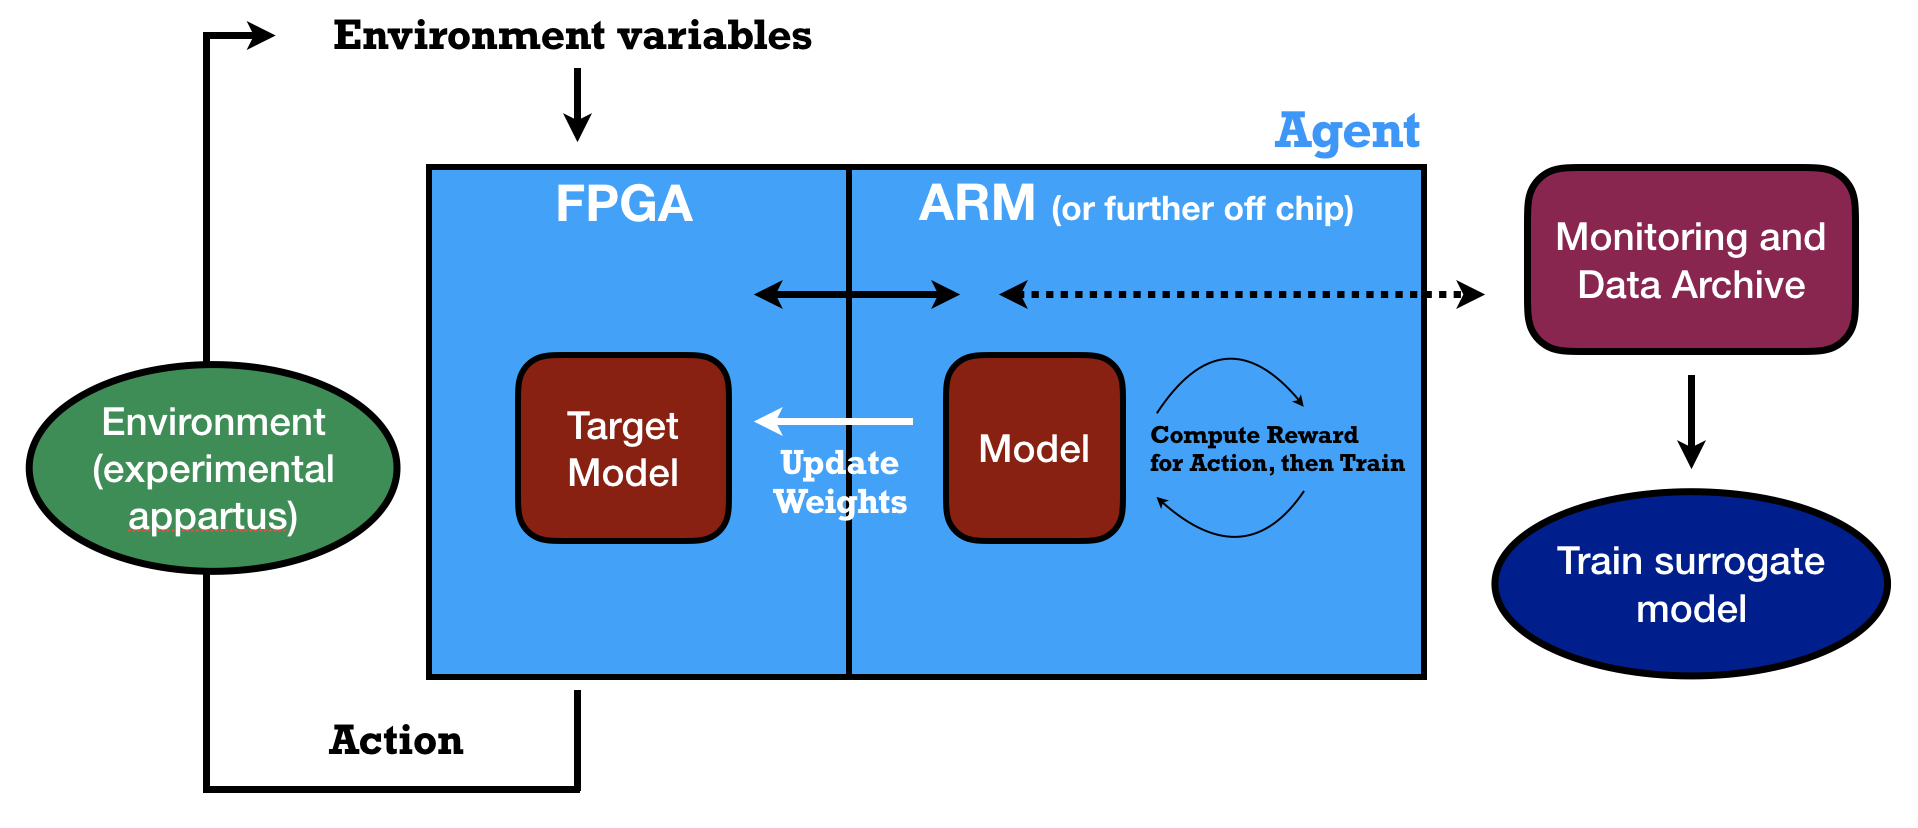
\includegraphics[keepaspectratio, width=0.6\textwidth]{proposal/img/reconfigurableArch.png}
  \caption{An example of a dynamically reconfigurable system}
  \label{fig:reinforce}
\vskip-10pt
\end{wrapfigure}
ML algorithms have been quite successfully implemented with digital hardware, so we do not plan to compete with the traditional, heavily resourced digital design companies, such as Intel and IBM, in developing AI and neuromorphic hardware. Nonetheless, commercial digital systems will have significant roles to play in AI\textsuperscript{3} research: in the short-, and mid-range goals, we plan to rely on digital platforms, such as FPGAs and digital ASICs, to realize the novel AI systems in this proposal. 

These systems will be co-designed with the algorithm developers and physics experimentalists in order to optimize their efficiency for the planned AI\textsuperscript{3} problems. As a result, AI\textsuperscript{3} will produce a stack of technologies for immediate, intermediate, and long-term solutions and workforce training. Our ability to span this stack of options will reduce the risks associated with each of these technologies when used alone. We plan to develop digital AI hardware that will be co-designed with the experiments to optimize the throughput and decision making in real-time.  To design the relevant AI algorithms that can be executed on our hardware, we plan to use and extend tools resulting from our research program, such as extensions to hlsfml~\cite{Duarte:2018ite} (see Section~\ref{sec:Programming}), for fast prototyping of algorithms. 
% add citations for Stewart, 2009; Bekolay, 2014; Lin, 2018]
%add citations to (Eliasmith, 2003, 2005)



\myparagraph{FPGA-based fast prototyping.} 


\myparagraph{Digital ASICs.}
ASICs are ideal for implementing integrated  on-detector low power and low latency edge computation. Power consumption due to data transfer from pixel to the chip periphery
%and subsequently off-chip 
dominates the total power consumed by ROICs. Hence locally analyzing data and extracting features not only efficiently utilizes data bandwidth, but also creates a smart detector.  There exist ASICs with highly parallel, modular sub-structures such as Google TPUs. However, co-design with the physics algorithms allows an extremely efficient, integrated, individually optimized kernel based approach for synthesizing complex interconnections. These interconnections allow extensive inter-regional (group of sensing elements) communication such that data analysis has a global view instead of just highly parallel local self-contained approach. 



\textbf{SP Memik} will lead the effort on implementing a holistic biologically-inspired retinomorphic approach where various individually optimized modules could be co-designed based on the AI algorithms. Designs will be fabricated in a fully depleted silicon-on-insulator (SOI) process (e.g. 22 FDX) for low power, high speed performance due to its lower parasitic capacitance. To achieve the ultimate power efficiency the digital circuits will be designed to operate in deep sub threshold regions with supply voltages of 200~mV or lower. Tool flows developed in Sec.~\ref{sec:Programming} will be utilized to convert AI algorithms to synthesizable Verilog for implementation. Standard CAD tools from vendors such as Cadence, Synopsys, Mentor Graphics etc. will be used to design, verify and create GDS II files for manufacture.  ASICs will be fabricated using dedicated multi-project wafer runs offered by several design aggregation service providers such as Globalshuttle, MOSIS, MUSE etc.





